\subsection{特異型EEJの分類}

特異型EEJは、その発生形態により以下の2つのタイプに分類される。

\subsubsection{未発達型 (Undeveloped type)}
EEJが十分に発達しておらず、赤道付近の観測点における電流強度が、赤道外の観測点におけるSq電流と同程度しか観測されないタイプである。


\subsubsection{突発型 (Sudden type)}
EEJが本来卓越するはずの正午付近（12:00 LT）において、赤道付近の観測点のEUELの値が急激に減少し、大きな落ち込みを見せるタイプである。
このタイプでは、日変化の形状が通常の放物線状とは大きく異なり、一時的な減少が特徴的である。

\begin{figure}[htbp]
  \centering
  \begin{minipage}{0.48\textwidth}
    \centering
    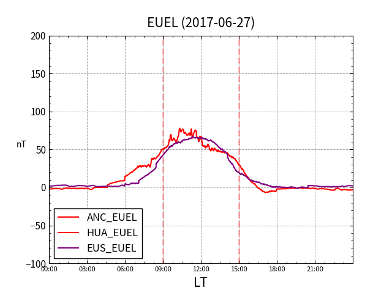
\includegraphics[width=\textwidth]{figures/undeveloped_type.png}
    \caption{未発達型EEJの例(2017-06-27)}
    \label{fig:undeveloped_type}
  \end{minipage}
  \hfill
  \begin{minipage}{0.48\textwidth}
    \centering
    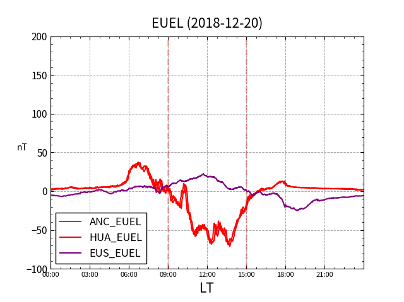
\includegraphics[width=\textwidth]{figures/sudden_type.png}
    \caption{突発型EEJの例(2018-12-20)}
    \label{fig:sudden_type}
  \end{minipage}
\end{figure}


